\chapter{Interprocess communication}

Write a C/C++ program which demonstrates interprocess communication between a reader process and a writer process. Use mkfifo, open, read, write and close APIs in your program.

\section{Description}

Pipes are the oldest form of UNIX System IPC and are provided by all UNIX systems. Pipes have two limitations.
\begin{enumerate}
	\item Historically, they have been half duplex (i.e., data flows in only one direction). Some systems now provide full-duplex 		pipes, but for maximum portability, we should never assume that this is the case.
	\item Pipes can be used only between processes that have a common ancestor. Normally, a pipe is created by a process, that 		process calls fork, and the pipe is used between the parent and the child.
\end{enumerate}

A pipe is created by calling the pipe function.
\begin{lstlisting}
	#include <unistd.h>
	int pipe(int filedes[2]);
\end{lstlisting}

\begin{lstlisting}
	Returns: 0 if OK, 1 on error
\end{lstlisting}

\begin{figure}[h!]
	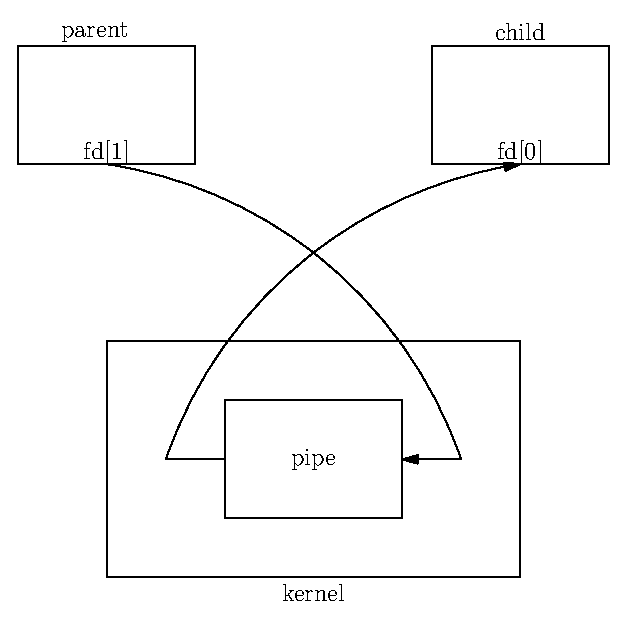
\includegraphics[width=\linewidth]{04IpcFifoReader/sample_box.eps}
	\caption{Pipe from parent to child}
\end{figure}
For a pipe from the child to the parent, the parent closes fd[1], and the child closes fd[0]. When one end of a pipe is closed, the following two rules apply.

\begin{enumerate}
	\item If we read from a pipe whose write end has been closed, read returns 0 to indicate an end of file after all the data 		has been read. (Technically, we should say that this end of file is not generated until there are no more writers for the 		pipe. It's possible to duplicate a pipe descriptor so that multiple processes have the pipe open for writing. Normally, 	however, there is a single reader and a single writer for a pipe. When we get to FIFOs in the next section, we'll see that 		often there are multiple writers for a single FIFO.)
	\item If we write to a pipe whose read end has been closed, the signal SIGPIPE is generated. If we either ignore the signal 		or catch it and return from the signal handler, write returns 1 with errno set to EPIPE.
\end{enumerate}

\begin{description}
\item 
	When we're writing to a pipe (or FIFO), the constant PIPE\_BUF specifies the kernel's pipe buffer size. A write of PIPE\_BUF bytes or less will not be interleaved with the writes from other processes to the same pipe (or FIFO). But if multiple processes are writing to a pipe (or FIFO), and if we write more than PIPE\_BUF bytes, the data might be interleaved with the data from the other writers. We can determine the value of PIPE\_BUF by using pathconf or fpathconf.
\end{description}

\section{Code}

\lstinputlisting[style=source-file]{04IpcFifoReader/04_read.cpp}
\lstinputlisting[style=source-file]{04IpcFifoReader/04_write.cpp}

\section{Output}

Run
\begin{lstlisting}[style=shell-command]
$ g++ 04_read.cpp -o 04_read.out
\end{lstlisting}
If no error, run
\begin{lstlisting}[style=shell-command]
$ g++ 04_write.cpp -o 04_write.out
\end{lstlisting}
If no error, run
\begin{lstlisting}[style=shell-command]
$ ./04_wite.out pipe1
\end{lstlisting}

Open another terminal without closong the first one
Change directory into the file location in the terminal
Run
\begin{lstlisting}[style=shell-command]
$ ./04_read.out pipe1
\end{lstlisting}
Shift to the original terminal and enter some string.
The same string should be displayed on the other terminal.

The output should be something like this
\begin{lstlisting}[style=shell-output]
Process 7685opening fifo in write mode
FD of fifo in write mode:3
enter data
	Test1
process 7685 finished writing
\end{lstlisting}

\begin{lstlisting}[style=shell-output]
FD of fifo in read mode:4196608
data read..
	Test1
process7915finished reading
\end{lstlisting}


